% hw3-unsupervised-learning.tex
\documentclass{article}
\usepackage{amsmath,algorithm2e,caption,subcaption,url,fullpage,graphicx}
\usepackage[authoryear,round]{natbib} 
\usepackage[usenames]{xcolor}
\usepackage{enumitem}
\usepackage{siunitx}

\bibliographystyle{plainnat}

\title{CS 4641: Machine Learning\\
Homework 3 --- Unsupervised Learning}
\date{}
\author{}

\begin{document}
\maketitle

\newcommand{\bphnote}[1]{\textit{\textcolor{red}{#1}}}


\section*{Instructions} 
\subsection*{Submission}
Please submit \textbf{one} zipfile containing a folder with \textbf{all} your code, data files, and a 
\textbf{single} pdf with your answers to the written questions. This zipfile should have the following format: 
\texttt{hw3-GTusername.zip}, replacing ``GTusername'' with your username (for example ``hw3-bhrolenok3.zip'').

For this assignment, your submission should include:
\begin{itemize}
	\item \texttt{hw3-answers.pdf} A PDF of your answers to the written questions.
	\item \texttt{hw3.py} The template file, modified to include your code.
	\item \texttt{README} Any special instructions for running your code, (library versions, network access, etc) 
	\textbf{plus} any external sources you used to help you with this assignment. This includes other students and websites. 
	When in doubt, cite it!
\end{itemize}

\subsection*{Collaboration}
All of the assignments in this class are \textbf{individual work only}. You're welcome to \emph{discuss} the math or high 
level concepts behind the algorithms you're being asked to implement, but you are 
\textbf{not allowed to share code or answers to the written questions}. We will be checking, manually and with automated 
tools, for any violations of this policy, so please \textbf{do not share solutions or code}.

\subsection*{Debugging tips}
In order to verify that your learners are working correctly, you can compare your results with those from a library such as \texttt{scikit-learn}\footnote{\url{https://scikit-learn.org/}}. For a quick debugging check, running the \texttt{main} method in the skeleton file should give you results for a simple debugging dataset that has only two dimensions, and should be easy to visualize. Figure \ref{fig:test-figs} shows the expected output for working PCA and \(k\)-Means implementations. The components found by PCA should be \([0.66, -0.75]^\top\) and \([0.75,0.66]^\top\) (sign flips are OK as long as the vectors are orthogonal). The cluster centers found by \(k\)-Means should be near \([-1.3,-1.7]^\top\) and \([1.5,1.5]^\top\). The reconstruction error when the number of components is the same as the original dimensionality should be close to zero for any dataset; for the test data the reconstruction error for 2 components is \(\num{3.1e-15}\).
\begin{figure}
\centering
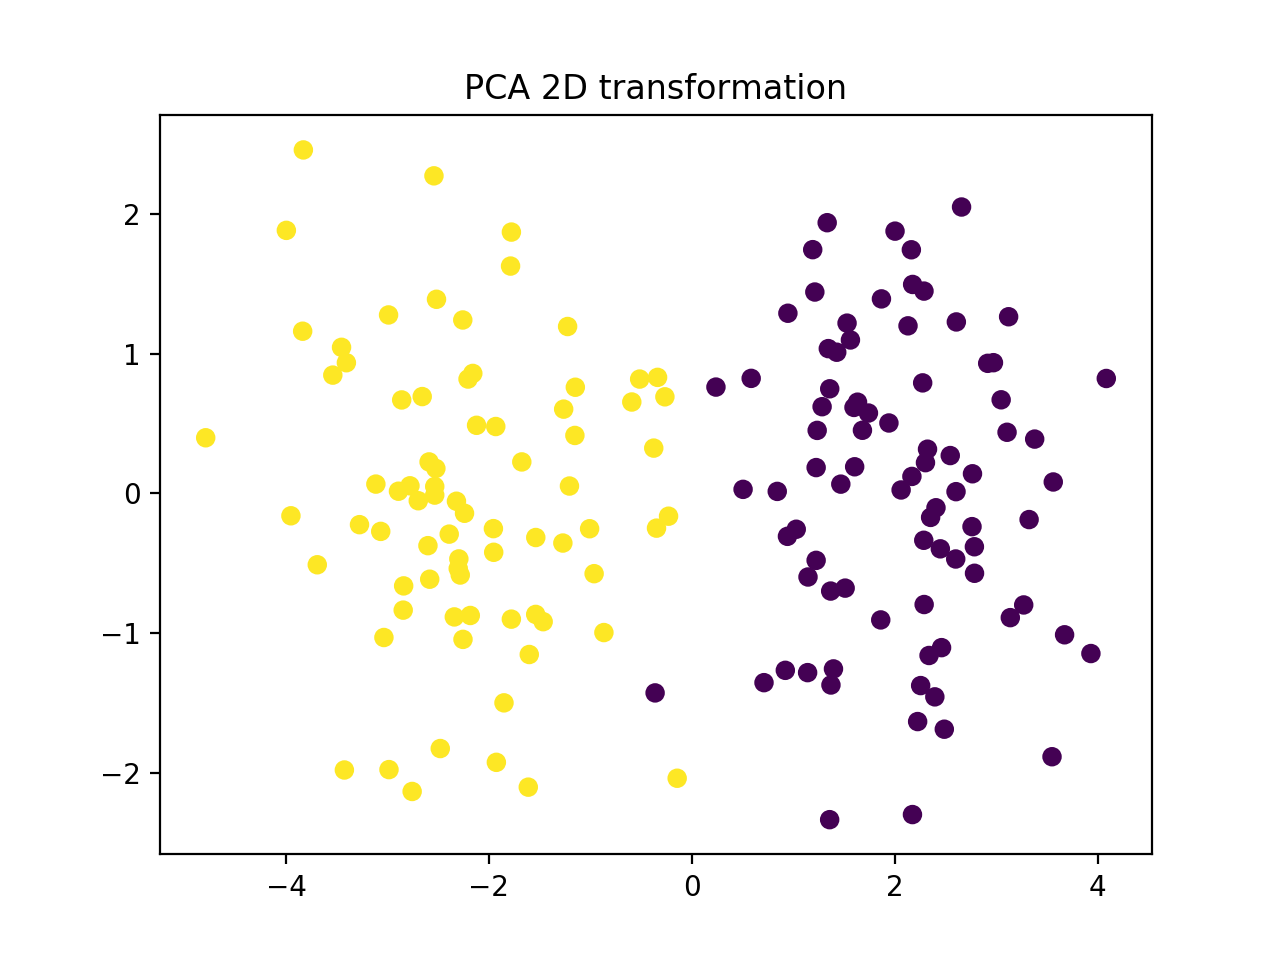
\includegraphics[width=0.4\textwidth]{pca-test-data}
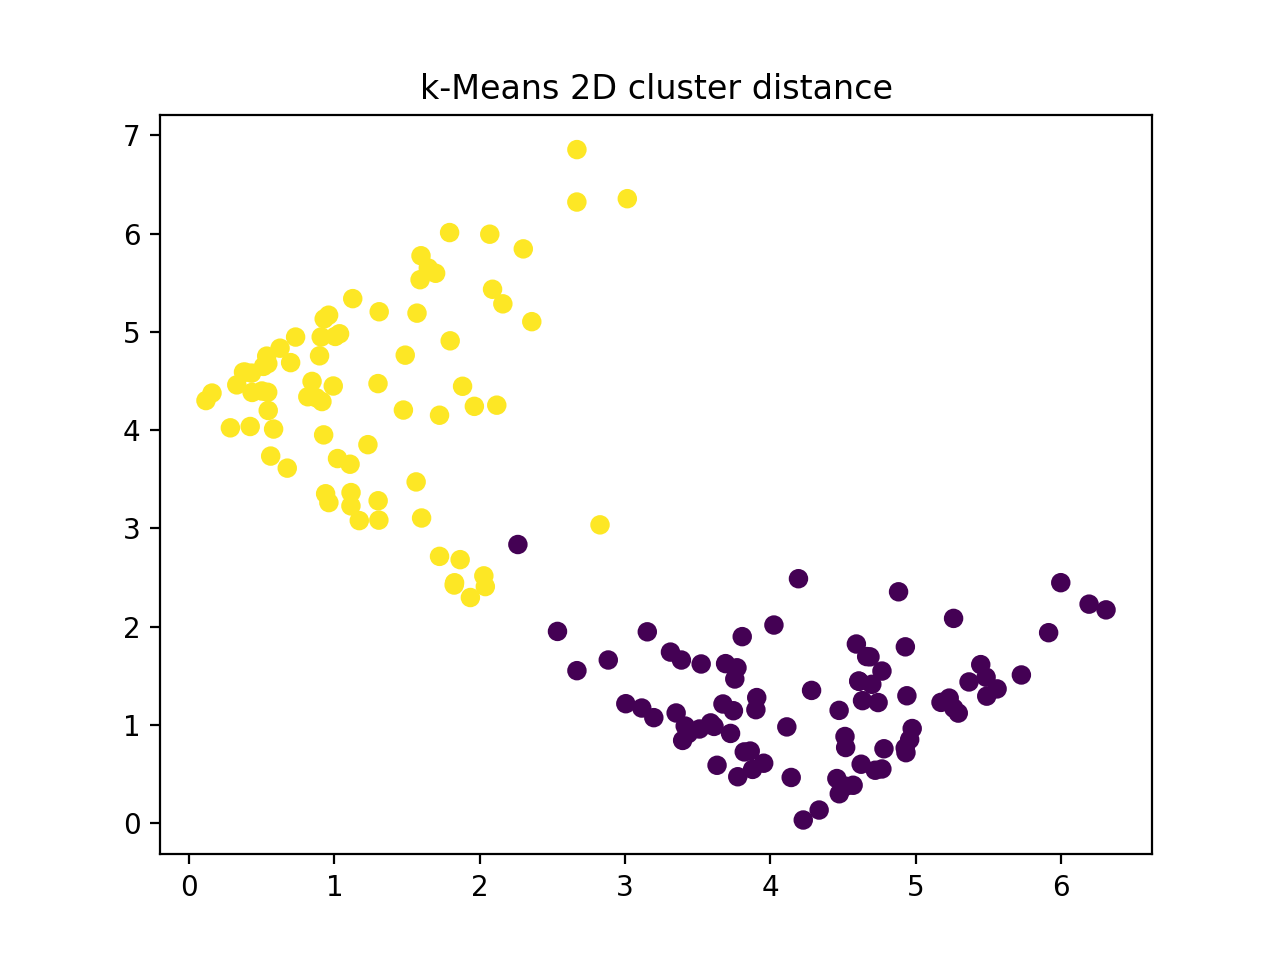
\includegraphics[width=0.4\textwidth]{km-test-data}
\caption{Expected output for PCA and \(k\)-Means on the 2D test dataset. The Normalized Mutual Information score should be close to \(0.95\).}
\label{fig:test-figs}
\end{figure}

\subsection*{Principal Component Analysis}
PCA is a very popular feature transformation technique that has nice theoretical properties and is still surprisingly simple to implement. The central method is based on the Singular Value Decomposition, which states that any matrix can be re-written as the product of three different matrices with useful properties:
\begin{align*}
	X &= U S V^\top
\end{align*}
For our purposes, the \(V\) matrix is the most interesting, because it contains as its columns the eigenvectors of the covariance matrix of \(X\), which as we showed in class, are exactly the vectors that point in the direction of ``highest variance.'' To actually solve for this decomposition, we can use the Numpy library, specifically the function \texttt{numpy.linalg.svd}. \textbf{Note 1}: read the documentation for this function carefully, so that you know what you need to pass in and what is being returned. Use this function to finish the implementation of \texttt{PCA.find\_components}, which should simply store the return values in the appropriate data members. \textbf{Note 2}: don't forget to center the data (subtract out the mean) before passing it to the \texttt{svd} function, otherwise your results may be different.

With the \(V\) matrix in hand, computing the actual feature transform is very simple. If \(X\) is the centered data, and \(V_L\) is the matrix consisting of the first \(L\) columns of \(V\), we can compute the transformed data \(X^\prime\) as follows:
\begin{align*}
	X^\prime &= X V_L
\end{align*}
Use this equation to implement the \texttt{PCA.transform} method, making sure to center the data, and only use the first \(L\) columns\footnote{This is easy to do using Numpy indexing. For a useful tutorial, see \url{https://docs.scipy.org/doc/numpy/reference/arrays.indexing.html}} of \(V\). For the final method you need to implement, we can leverage one of the special properties of \(V\), namely that \(V^\top = V^{-1}\). This means we can write the \emph{inverse} transform as:
\begin{align*}
	X^{\prime\prime} &= X^\prime V_L^\top
\end{align*}
Implement this in \texttt{PCA.inv\_transform} to complete the class, making sure to ``undo'' the centering you did in the original transform (add the mean back in)\footnote{Note that unless \(V_L=V\) (we use all of the columns of V), the reconstructed \(X^{\prime\prime}\) won't necessarily exactly equal \(X\). This difference is what \texttt{PCA.reconstruction\_error} measures.}. With all three of these methods finished, your PCA implementation should be complete, and you can test out the plotting methods provided for you to visualize any high dimensional dataset by projecting it down to the first two or three principal components. You can also see how much ``information'' is lost in these projections by looking at the reconstruction error, which is the difference between the original data, and the data passed through a low-dimensional transform and then re-projected back to the original space. This is implemented for you in \texttt{PCA.reconstruction\_error}.

\subsection*{\(k\)-Means clustering}
\(k\)-Means clustering is a simple iterative method for finding clusters that alternates between assigning clusters to centers, and recomputing center locations given assigned points. Formally, we can describe the process as follows:

\begin{algorithm}[H]
	\SetAlgoLined
	\KwData{number of clusters \(K\), data \(\{\mathbf{x}^{(i)}\}_{i=1}^N\)}
	\KwResult{cluster centers, \(\{\mathbf{c}^{(k)}\}_{k=1}^K\)}
	Initialize each \(\mathbf{c}^{(k)}\) to a randomly chosen \(\mathbf{x}^{(i)}\)\\
	\While{not done}{
		Assign each \(\mathbf{x}^{(i)}\) to the closest \(\mathbf{c}^{(k)}\)\\
		Set each \(\mathbf{c}^{(k)}\) to be the average of all the \(\mathbf{x}^{(i)}\) assigned to it\\
		If cluster assignments did not change, done
	}
	~
\end{algorithm}

Implement this algorithm in \texttt{KMeans.cluster}. Note that detecting whether cluster assignments have changed can be tricky if there are ties in the distances, so you may want to make use of the helper function \texttt{consistent\_ordering}, or you may want to handle this in your own way.

Once you've implemented this method, the \texttt{KMeans} class should be complete. Typically, the cluster centers are what we're after in \(k\)-Means clustering, but these can be used in a variety of different ways. If the purpose is feature reduction/transformation, we can use distance to the discovered clusters as a new set of features. This is how the provided 2D and 3D plotting functions work: they first find two/three clusters, then transform the data into this new space, which can then be used as a visualization of the high dimensional data. 

Alternatively, if visualization isn't the goal we can instead label each point with the closest cluster center, and then use the cluster centers themselves as a kind of ``summary'' of the data. It's difficult to come up with good measures of clustering performance when all we have is the data itself, but thankfully for each of the provided datasets we also have an actual class label (even though we ignored it when clustering). One way to measure cluster performance when we have access to this class label data is by measuring the Mutual Information between the cluster labels and the class labels. If the clusters do a good job of summarizing the data, then they should have a strong statistical relationship with the class labels. The standard statistical formula for measuring this kind of relationship is known as Mutual Information, and it's defined to be
\begin{align*}
	MI(U,V) &= \sum_i\sum_j p(U_i,V_j) \cdot \log\frac{p(U_i,V_j)}{p(U_i)\cdot p(V_j)}
\end{align*}
where \(p(U_i,V_j)\) is the joint probability of a datapoint having both cluster label \(i\) and class label \(j\), while \(p(U_i)\) and \(p(V_j)\) are the respective marginal probabilities for cluster label \(i\) and class label \(j\). The max and min values of Mutual Information are dependent on the number of class and cluster labelings, so this equation is often normalized to be a value between 0 and 1, with values near 0 having a weak relationship, and values near 1 having a strong relationship. This normalized version is implemented for you in \texttt{KMeans.normalized\_mutual\_information}. Try this out on the testing dataset with two clusters and you should see a Normalized Mutual Information very close to 1, indicating that the cluster labels agree with the class labels.

\section*{Questions}
\begin{enumerate}
	\item PCA
	\begin{enumerate}
		\item Run PCA on the three datasets, \texttt{iris}, \texttt{HTRU2}, and \texttt{digits}. For each dataset, visualize the 2D and 3D projections of the training data (6 graphs). Make sure each point is colored according to its class label (see the ``with labels'' example in the template main function).
		\item If we were to use PCA to transform the original features into those visualized in the previous question, do you think it would improve, reduce, or have no effect on performance if you were using Logistic Regression to classify the transformed data? Explain your reasoning. Answer for both 2D and 3D for each of the three datasets.
	\end{enumerate}
	\item \(k\)-Means
	\begin{enumerate}
		\item Use \(k\)-Means as a feature transform, and visualize the transformed data in 2D and 3D for each of the three datasets (like you did for PCA). Again, use the ``with labels'' version so that the class label of each point is clear.
		\item Compare \(k\)-Means to PCA as a \emph{feature transform} for each of the three datasets. Do you think it would be better to use PCA or \(k\)-Means to transform the data into 2D and 3D? Specifically, do you think it would be better in terms of classification performance on the transformed data? Explain your reasoning, and answer for both 2D and 3D for each dataset.
		\item The primary use for \(k\)-Means is not as a feature transform, but as a clustering method. Use the Normalized Mutual Information metric, described above, to get a quantitative measure of cluster quality when using the same number of clusters as classes for each of the three datasets. Report the performance on the training data, and explain why you got the results you did.
	\end{enumerate}
	\item Bayes Nets
	\begin{enumerate}
		\item Consider the following four random variables: \(Cough, Fever, Allergies, Flu\). You know that a cough can be caused by either allergies or the flu, fever can only be caused by the flu, and allergies and the flu have no causal relationship. Draw a Bayes Net that represents this set of random variables and their independence/dependence relationships.
		\item Using the Bayes Net from the previous question, write down how you would factor the joint probability distribution, \(p(Cgh,Fev,Alg,Flu)\), as a product of conditional probabilities and marginals given by the Bayes Net.
		\item In standard Hidden Markov Models, the three distributions you need to do any of the inference tasks we talked about (filtering, smoothing, prediction, learning) are the \emph{transition model}:
		\begin{align*}
			p(Z_t=k\mid Z_{t-1}=j) &= A_{jk}
		\end{align*}
		the \emph{observation model}:
		\begin{align*}
			p(X_t=l\mid Z_t =j) &= B_{jl}
		\end{align*}
		and the \emph{prior}:
		\begin{align*}
			p(Z_0=j) &= \pi_j
		\end{align*}
		A simple modification of HMMs called Input/Output HMMs (or IOHMMs) changes the assumptions slightly. Instead of assuming transitions between hidden states are completely hidden, the model assumes that transitions can be at least partially influenced by some observable random variable, \(U_t\). The Bayes Net for this model is given in Figure \ref{fig:iohmm-bn}. Under the IOHMM model, what distributions do you need? Describe them precisely in probability notation as was done above for HMMs.
		\item In class we talked about how observing a common effect can make two marginally independent random variables not conditionally independent (conditioned on the common effect). A simple example of this is the \texttt{XOR} function on two bits. Let \(X_1\) and \(X_2\) be random variables that take the values \(1\) or \(0\) with equal probability, and let \(Y\) be a random variable which is the \texttt{XOR} of \(X_1\) and \(X_2\). Show that, given \(Y\), the joint probability of \(X_1\) and \(X_2\) is not the same as the product of \(X_1\) given \(Y\) and \(X_2\) given \(Y\). That is, show that
		\begin{align*}
			p(X_1, X_2\mid Y) &\neq p(X_1\mid Y)\cdot p(X_2\mid Y)
		\end{align*} 
		For reference, the Bayes Net for this problem is given in Figure \ref{fig:hw3-bn}.
	\end{enumerate}
\end{enumerate}
\begin{figure}
\centering
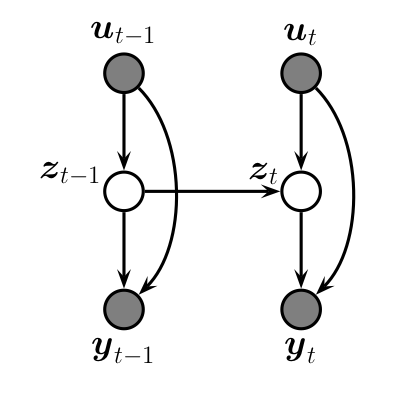
\includegraphics[height=0.3\textheight]{LDS-UZY}
\caption{Bayes Net for IOHMMs.}
\label{fig:iohmm-bn}
\end{figure}
\begin{figure}
\centering
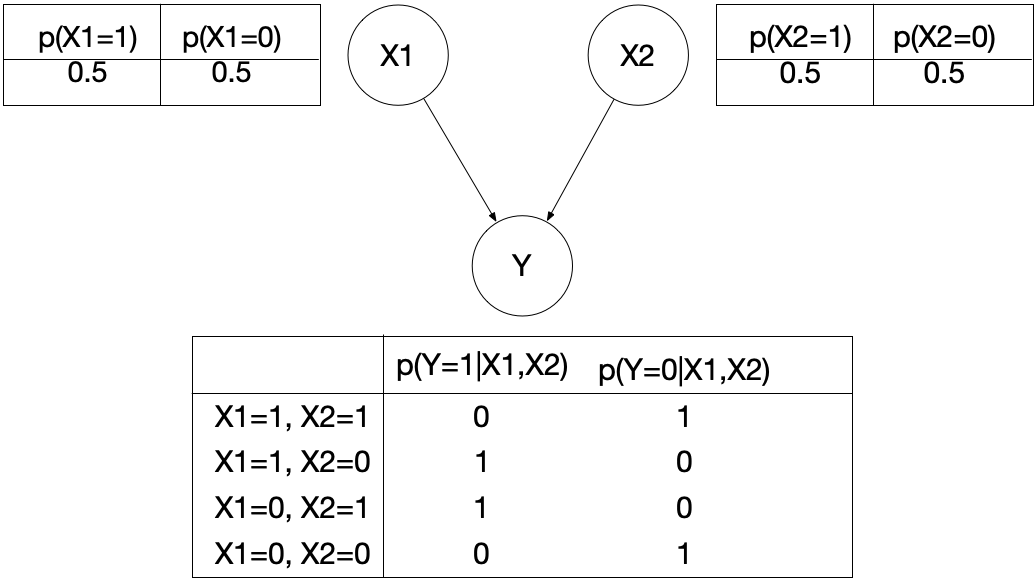
\includegraphics[height=0.3\textheight]{ml-hw3-bayes}
\caption{Bayes Net for the \texttt{XOR} question.}
\label{fig:hw3-bn}
\end{figure}
\end{document}